\chaplbl{Teaching as a Performance Art}{s:performance}

Continuing with our theme of instructor-as-performer, let's discuss some
research that suggests that improvement in educational outcomes must be
driven by practice and communities of practice. The tricks and
techniques that make teaching effective cannot be mandated from above,
but will develop into widespread effectiveness only as they are shared
through a community of teaching practice.

\seclbl{Lesson Study}{sec:lesson-study}

Many people assume that teachers are born, not made. From politicians to
researchers and teachers themselves, most reformers have designed
systems to find and promote those who can teach and eliminate those who
can't. As Elizabeth Green describes in
\textit{Building a Better Teacher} \cite{bib:green-babt}, though,
that assumption is wrong, which is why
educational reforms based on it have repeatedly failed.

The book is written as a history of the people who have put that puzzle
together in the US. Its core begins with a discussion of what James
Stigler discovered during a visit to Japan in the early 1990s:

\begin{quote}
Some American teachers called their pattern ``I, We, You'': After
checking homework, teachers announced the day's topic, demonstrating a
new procedure (I)\ldots{} Then they led the class in trying out a sample
problem together (We)\ldots{} Finally, they let students work through
similar problems on their own, usually by silently making their way
through a worksheet (You)\ldots{}

The Japanese teachers, meanwhile, turned ``I, We, You'' inside out. You
might call their version ``You, Y'all, We.'' They began not with an
introduction, but a single problem that students spent ten or twenty
minutes working through alone (You)\ldots{} While the students worked,
the teacher wove through the students' desks, studying what they came up
with and taking notes to remember who had which idea. Sometimes the
teacher then deployed the students to discuss the problem in small
groups (Y'all). Next, the teacher brought them back to the whole group,
asking students to present their different ideas for how to solve the
problem on the chalkboard\ldots{} Finally, the teacher led a discussion,
guiding students to a shared conclusion (We).
\end{quote}

It's tempting but wrong to think that this particular teaching technique
is Japan's secret sauce. The actual key is revealed in the description
of Akihiko Takahashi's work. In 1991, he visited the United States in a
vain attempt to find the classrooms described a decade earlier in a
report by the National Council of Teachers of Mathematics. He couldn't
find them. Instead, he found that American teachers met once a year (if
that) to exchange ideas about teaching, compared to the weekly or even
daily meetings he was used to. What was worse:

\begin{quote}
The teachers described lessons they gave and things students said, but
they did not \emph{see} the practices. When it came to observing actual
lessons---watching each other teach---they simply had no
opportunity\ldots{} They had, he realized, no \emph{jugyokenkyu}.
Translated literally as ``lesson study'', \emph{jugyokenkyu} is a bucket
of practices that Japanese teachers use to hone their craft, from
observing each other at work to discussing the lesson afterward to
studying curriculum materials with colleagues. The practice is so
pervasive in Japanese schools that it is\ldots{}effectively invisible.

And here lay the answer to {[}Akihiko's{]} puzzle. Of course the
American teachers' work fell short of the model set by their best
thinkers\ldots{} Without \emph{jugyokenkyu}, his own classes would have
been equally drab. Without \emph{jugyokenkyu}, how could you even teach?
\end{quote}

So what does \emph{jugyokenkyu} look like in practice?

\begin{quote}
In order to graduate, education majors not only had to watch their
assigned master teacher work, they had to effectively replace him,
installing themselves in his classroom first as observers and then, by
the third week, as a wobbly\ldots{}approximation of the teacher himself.
It worked like a kind of teaching relay. Each trainee took a subject,
planning five days' worth of lessons\ldots{} {[}and then{]} each took a
day. To pass the baton, you had to teach a day's lesson in every single
subject: the one you planned and the four you did not\ldots{} and you
had to do it right under your master teacher's nose. Afterward,
everyone---the teacher, the college students, and sometimes even another
outside observer---would sit around a formal table to talk about what
they saw.

{[}Trainees{]} stayed in\ldots{}class until the students left at 3:00
pm, and they didn't leave the school until they'd finished discussing
the day's events, usually around eight o'clock. They talked about what
{[}the master teacher{]} had done, but they spent more time poring over
how the students had responded: what they wrote in their notes; the
ideas they came up with, right and wrong; the architecture of the group
discussion. The rest of the night was devoted to planning\ldots{}

\ldots{}By the time he arrived in {[}the US{]}, {[}Akihiko had{]}
become\ldots{}famous\ldots{} giving public lessons that attracted
hundreds, and, in one case, an audience of a thousand. He had a
seemingly magical effect on children\ldots{} But Akihiko knew he was no
virtuoso. ``It is not only me,'' he always said\ldots{} ``\emph{Many}
people.'' After all, it was his mentor\ldots{}who had taught him the new
approach to teaching\ldots{} And {[}he{]} had crafted the approach along
with the other math teachers in {[}his ward{]} and beyond. Together, the
group met regularly to discuss their plans for teaching\ldots{} {[}At{]}
the end of a discussion, they'd invite each other to their classrooms to
study the results. In retrospect, this was the most important lesson:
not how to give a lesson, but how to study teaching, using the cycle of
\emph{jugyokenkyu} to put\ldots{}work under a microscope and improve it.
\end{quote}

Putting work under a microscope in order to improve it is commonplace in
sports and music. A professional musician, for example, will dissect
half a dozen different recordings of ``Body and Soul'' or ``Smells Like
Teen Spirit'' before performing it. They would also expect to get
feedback from fellow musicians during practice and after performances.
Many other disciplines work this way too: the Japanese drew inspiration
from \href{https://en.wikipedia.org/wiki/W.\_Edwards\_Deming}{Deming}'s
ideas on continuous improvement in manufacturing, while the adoption of
code review over the last 15 years has done more to improve everyday
programming than any number of books or websites.

But this kind of feedback isn't part of teaching culture in
English-language school systems: in the US, Canada, the UK, Australia,
and elsewhere, what happens in the classroom stays in the classroom.
Teachers don't watch each other's lessons on a regular basis, so they
can't borrow each other's good ideas. The result is that \emph{every
teacher has to invent teaching on their own}. They may get lesson plans
and assignments from colleagues, the school board, a textbook publisher,
or the Internet, but each teacher has to figure out on their own how to
combine that with the theory they've learned in education school to
deliver an actual lesson in an actual classroom for actual students.

Fincher and her colleagues studied how teaching practices are actually
transferred using both a detailed case study \cite{bib:fincher-warrens-questions}
and analysis of change stories \cite{bib:fincher-stories-change}.
The abstract of the latter paper sums up their findings:

\begin{quote}
Innovative tools and teaching practices often fail to be adopted by
educators in the field, despite evidence of their effectiveness. Naïve
models of educational change assume this lack of adoption arises from
failure to properly disseminate promising work, but evidence suggests
that dissemination via publication is simply not effective\ldots{} We
asked educators to describe changes they had made to their teaching
practice and analyzed the resulting stories\ldots{} Of the 99 change
stories analyzed, only three demonstrate an active search for new
practices or materials on the part of teachers, and published materials
were consulted in just eight of the stories. Most of the changes
occurred locally, without input from outside sources, or involved only
personal interaction with other educators.
\end{quote}

Barker et al found something similar in 2015 \cite{bib:barker-practice-adoption}:

\begin{quote}
Adoption is not a ``rational action,'' however, but an iterative series
of decisions made in a social context, relying on normative traditions,
social cueing, and emotional or intuitive processes\ldots{}
{[}F{]}aculty are not likely to use educational research findings as the
basis for adoption decisions. Faculty become aware of innovative
practices either because a problem leads them to intentionally seek them
out, or they hear about them through funded initiatives, conferences and
journals, or from colleagues. They experiment (or not) for several
reasons, depending on institutional expectations and policies, perceived
costs and benefits for themselves and students, and the influence of
role models. Faculty tend to trust other faculty whose work and
institutional context is more like their own. The choice to try out
practices competes with the need to ``cover'' material, as well as with
classroom layouts. Positive student feedback is taken as strong evidence
by faculty that they should continue a practice.
\end{quote}

\begin{callout}{Learning Sideways}{callout:learning-sideways}

The phrase \emph{lateral knowledge transfer} is sometimes used to
describe what happens when someone intended to teach one thing, but
their audience learned another along the way. For example, an instructor
might set out to show people how to do a particular statistical analysis
in R, but what her learners might take away is some new keyboard
shortcuts in R Studio. Live coding makes this much more likely because
it allows learners to see the ``how'' as well as the ``what''.
\end{callout}

\begin{challenge}{Giving Feedback}{chal:giving-feedback}

Watch \href{https://www.youtube.com/watch?v=-ApVt04rB4U}{this video} as
a group and then give feedback on it. Try to organize feedback along two
axes: positive vs.~negative and content (what was said) vs.~presentation
(how it was said).
\end{challenge}

\begin{challenge}{Feedback on Yourself}{chal:feedback-on-yourself}

\begin{enumerate}
\item
  Split into groups of three
\item
  Have each person introduce themselves and then explain, in no more
  than 90 seconds, the key idea or ideas from the Carpentry lesson
  episode they chose before the start of the training course to another
  person in the group while the third person records it (video and
  audio) using a cell phone or some other handheld device.
\item
  After the first person finishes, rotate roles (she becomes the
  videographer, her audience becomes the instructor, the person who was
  recording becomes the audience) and then rotate roles again.
\item
  After everyone in the group of three has finished teaching, watch the
  videos as a group. Everyone gives feedback on all three videos, i.e.,
  people give feedback on themselves as well as on others.
\item
  After everyone has given feedback on all of the videos, return to the
  main group and put everyone's feedback about you into the Etherpad.
\end{enumerate}
\end{challenge}

\seclbl{On Stage}{sec:on-stage}

\begin{discussion}{What Are Your Tells?}{disc:what-are-your-tells}

How was the experience of being videoed/receiving feedback? What did
people notice? What are some of your ``tells''?
\end{discussion}

Everyone has nervous habits. While these habits are often not as
noticeable as you would think, it's good to identify ways to keep
yourself from pacing, or fiddling with your jewellery, or not looking at
the audience. For example, many of us become ``Mickey Mouse'' versions
of ourselves when we're nervous, i.e., we talk more rapidly than usual,
in a higher-pitched voice, and wave our arms around more than we usually
would.

But just like everyone has their own nervous habit, each person has
their own strengths. Musicians can be very different (but equally
effective!) in their performance of the same piece; similarly, teachers
can present the same material in very different ways. The uniqueness of
your teaching style can and should be based on your strengths. This is
why it's just as important to identify strengths as weaknesses when
trying to improve your teaching. It's good to know what you do well!

\seclbl{Feedback}{sec:feedback}

Sometimes it can be hard to receive feedback, especially negative
feedback.

\begin{figure}[htbp]
\centering
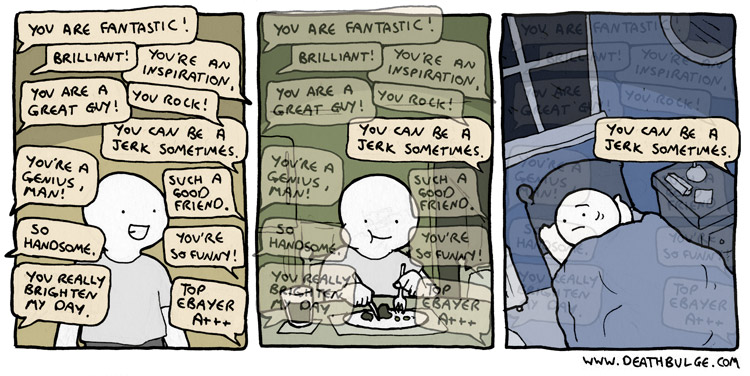
\includegraphics{../fig/deathbulge-jerk.jpg}
\caption{Feedback Feelings}
\end{figure}

Feedback is most effective when the people involved can share ground
rules and expectations. This is especially important when the instructor
and/or students have different cultural or domain expectations about
feedback.

Here is a list of different ways that you, as the instructor, can set
the stage for receiving feedback in a way that helps you improve:

\begin{itemize}
\item
  Initiate feedback. It's better to ask for feedback than to receive it
  unwillingly.
\item
  Choose your own questions and ask for specific feedback. For example:

  \begin{itemize}
    \item
    ``What is one thing I could have done as an instructor to make this
    lesson more effective?''
  \item
    ``If you could pick one thing from the lesson to go over again, what
    would it be?''
  \end{itemize}
\end{itemize}

Specific feedback like this is more useful than a generic ``that was
great!'' or ``that was terrible!'' Also, writing your own feedback
questions allows you to frame feedback in a way that is helpful to you -
the questions above reveal what didn't work in your teaching, but read
as professional suggestions rather than personal judgments.

\begin{itemize}
\item
  Communicate expectations. If your teaching feedback is taking the form
  of an observation (and you're comfortable enough with the observer),
  tell that person how they can best communicate their feedback to you.
\item
  Balance positive and negative feedback.

  \begin{itemize}
    \item
    Ask for or give ``compliment sandwiches'' (one positive, one
    negative, one positive)
  \item
    Ask for both types of feedback
  \end{itemize}
\item
  Use a feedback translator. Have a fellow instructor (or other trusted
  person in the room) read over all the feedback and give an executive
  summary. It can be easier to hear ``It sounds like most people are
  following, so you could speed up'' than to read several notes all
  saying, ``this is too slow'' or ``this is boring''.
\end{itemize}

This is part of the reason for Data Carpentry and Software Carpentry's
rule, ``Never teach alone.'' Having another instructor in the classroom
saves your voice (it's hard to talk for two days straight), but more
importantly, it's a chance for instructors to learn from one another and
be a supportive voice in the room.

Finally, be kind to yourself. Mental habits matter: if you're a
self-critical person, it's OK to remind yourself that:

\begin{itemize}
\item
  It's not personal.
\item
  Look at the positives along with the negatives.
\item
  Etc.
\end{itemize}

\begin{challenge}{Feedback on Feedback}{chal:feedback-on-feedback}

Watch either \href{https://vimeo.com/139316669}{this video} or
\href{https://vimeo.com/139181120}{this one}. Take notes about
the presentation, and divide those into four groups based on whether
they are positive or negative and whether they are about the content
(what was said) or the presentation (how it was said, e.g., body
language). Compare your notes with those made by other people, and with
the feedback given by your instructor.
\end{challenge}

\begin{challenge}{Feedback on Yourself, Part II}{chal:feedback-on-yourself-part-ii}

Later in the training, repeat the first challenge exercise; however,
when it comes time to give feedback, use the same 2x2 scheme in the
previous challenge.
\end{challenge}

\begin{challenge}{Learn More About Feedback}{chal:learn-more-about-feedback}

Read Gormally et al's
``Feedback about Teaching in Higher Ed'' \cite{bib:gormally-teaching-feedback}
and discuss ways you could make peer-to-peer feedback a routine part of your teaching.
You may also enjoy Gawande's ``Personal Best'' \cite{bib:gawande-personal-best},
which looks at the value of having a coach.
\end{challenge}

\begin{challenge}{Fill In Minute Cards}{chal:fill-in-minute-cards}

We frequently use sticky notes as \emph{minute cards}: before each
break, learners take a minute to write one positive thing on the green
sticky note (e.g., one thing they've learned that they think will be
useful), and one thing they found too fast, too slow, confusing, or
irrelevant on the red one. They can use the red sticky note for
questions that haven't yet been answered. While they are enjoying their
coffee or lunch, the instructors review and cluster these to find
patterns. It only takes a few minutes to see what learners are enjoying,
what they still find confusing, what problems they're having, and what
questions are still unanswered.

Write one thing you learned this morning that you found useful on your
green sticky note, and one question you have about the material on the
red. Do \emph{not} put your name on the notes: this is meant to be
anonymous feedback. Add your notes to the pile by the door as you leave
to get coffee.
\end{challenge}
